\documentclass[11pt,a4paper,oneside]{memoir}

\usepackage{graphicx}
\usepackage{geometry}
\usepackage{float}
\usepackage{hyperref}
\usepackage[table]{xcolor}
\usepackage[backend=biber,style=numeric,maxnames=4]{biblatex}
\usepackage{tabularx}
\usepackage{acro}
\usepackage{textcomp}

\newcolumntype{L}{>{\raggedright\arraybackslash}X}
\newcolumntype{C}{>{\centering\arraybackslash}X}
\def\tabularxcolumn#1{m{#1}}

\addbibresource{bibliography.bib}

\hypersetup{
	colorlinks=true,
	linkcolor=black,
	urlcolor=blue,
	citecolor=black,
}

\graphicspath{{figures/}}

\setsecnumdepth{subsection}

%\setcounter{tocdepth}{2}

\acsetup{make-links}

\DeclareAcronym{sw}{
	short=SW,
	long=Software,
}

\DeclareAcronym{hw}{
	short=HW,
	long=Hardware,
}

\DeclareAcronym{fsm}{
	short=FSM,
	long=Finite-State Machine,
}

\DeclareAcronym{hdl}{
	short=HDL,
	long=\acl{hw} Description Language,
}

\DeclareAcronym{rtl}{
	short=RTL,
	long=Register-Transfer Level
}

\DeclareAcronym{hls}{
	short=HLS,
	long=High-Level Synthesis,
}

\DeclareAcronym{fpga}{
	short=FPGA,
	long=Field-Programmable Gate Array,
}

\DeclareAcronym{fifo}{
	short=FIFO,
	long=First-In First-Out,
}

\DeclareAcronym{lru}{
	short=LRU,
	long=Least Recently Used,
}

\DeclareAcronym{ram}{
	short=RAM,
	long=Random Access Memory,
	long-plural-form=Random Access Memories,
}

\DeclareAcronym{dram}{
	short=DRAM,
	long=Dynamic \acs{ram},
}

\DeclareAcronym{bram}{
	short=BRAM,
	long=Block \acs{ram},
}

\DeclareAcronym{axi}{
	short=AXI,
	long=Advanced eXtensible Interface,
}

\DeclareAcronym{raw}{
	short=RAW,
	long=Read After Write,
}

\DeclareAcronym{ii}{
	short=II,
	long=Initiation Interval,
}

\DeclareAcronym{sfinae}{
	short=SFINAE,
	long=Substitution Failure Is Not An Error,
}

\DeclareAcronym{l1}{
	short=L1,
	long=Level 1,
}

\DeclareAcronym{l2}{
	short=L2,
	long=Level 2,
}

\DeclareAcronym{api}{
	short=API,
	long=Application Programming Interface,
}

\renewcommand*{\maketitle}%
{
	\newgeometry{left=2cm,right=2cm,top=3cm,bottom=3.5cm}

	\begin{center}
		\begingroup
		{\Huge\textbf{POLITECNICO DI TORINO}}\\[\baselineskip]
		\rule{\textwidth}{2pt}\par
		\vspace*{1em}
		{\LARGE\textbf{Master's Degree in Computer Engineering}}\\[\baselineskip]
		\vspace*{1em}
		{\Large\textbf{Master's Degree Thesis}}\\
		\vspace*{2cm}
		{\huge\textbf{Acceleration by Separate-Process Cache for
		Memory-Intensive Algorithms on \acs{fpga} via \acl{hls}}}\\
		\vspace*{1cm}
		
\includegraphics[width=.3\textwidth]{figures/polito-logo}
	\end{center}
	\vfill
	\begin{minipage}{0.4\textwidth}
		\begin{flushleft}
			{\Large
				\textbf{Supervisor}\\
				Prof.\ Luciano Lavagno
			}
		\end{flushleft}
	\end{minipage}
	\begin{minipage}{0.4\textwidth}
		\begin{flushright} 
			{\Large
				\textbf{Candidate}\\
				Giovanni Brignone\\
				ID: 274148
			}
		\end{flushright}
	\end{minipage}  
	\vspace*{2cm}
	\begin{center}
		{\Large\textbf{Academic year 2020-2021}}
	\end{center}
	\endgroup

	\restoregeometry 
}

\begin{document}
\pagestyle{empty}
\maketitle

\frontmatter
\chapter*{Abstract}
The end of the Moore's Law validity is making the performance advance of
\acl{sw} run on general purpose processors more challenging than ever.
Since current technology cannot scale anymore it is necessary to approach the
problem from a different point of view: application-specific \acl{hw} can
provide higher performance and lower power consumption, while requiring higher
design efforts and higher deployment costs.

The problem of the high design efforts can be mitigated by the \acf{hls}, since
it helps improving designer productivity thanks to convenient \acl{sw}-like
tools.

The problem of high deployment costs can be tackled with \acp{fpga}, which allow
to implement special-purpose \acl{hw} modules on general-purpose underlying
physical architectures.

\bigskip
One of the open issues of \ac{hls} is the memory bandwidth bottleneck which
limits performance, especially critical in case of memory-bound algorithms.

\acp{fpga} memory system is composed of three main kind of resources: registers,
\acp{bram} and external \acp{dram}.
Current \ac{hls} tools allow to exploit this memory hierarchy manually, in a
scratchpad-like fashion: the objective of this thesis work is to automate the
memory management by providing a easily integrable and fully customizable cache
system for \ac{hls}.

\bigskip
The proposed implementation has been developed using Vitis\texttrademark HLS
tool by Xilinx Inc..

The first development phase produced a single-port cache module, in the form of
a C++ class configurable through templates in terms of number of sets, ways,
words per line and replacement policy.
The cache lines have been mapped to \acp{bram}.
To obtain the desired performance an unconventional (for \ac{hls}) multi-process
architecture has been developed: the cache module is a separate process with
respect to the algorithm using it: the algorithm logic sends a memory access
request to the cache and reads its response, communicating through \acsp{fifo}.

\bigskip
In the second development phase the focus was put on performance optimization,
in two dimensions: increasing the memory hierarchy depth by introducing a
\ac{l1} cache and increasing parallelism by enabling multiple ports.

The \ac{l1} cache is composed of cache logic inlined in the user algorithm: this
solution allows to cut the costs of \acp{fifo} communications. To keep \ac{l1}
cache simple it has been implemented with a write-through write policy,
therefore it provides advantages for read accesses only. It is configurable in
the number of lines and each line contains the same number of words of the
associated \ac{l2} cache.

The multi-port solution provides a single \ac{l2} cache accessible from multiple
\acp{fifo} ports, each of which can be associated with a dedicated \ac{l1}
cache.
It is possible to specify the number of ports through a template parameter and
it typically corresponds to the unroll factor of the loop in which the cache
is accessed.

\bigskip
In order to evaluate performance and resource usage impact of the developed
cache module, multiple algorithms with different memory access patterns have
been synthesized and simulated, with all data accessed to \ac{dram} (performance
lower bound), to \ac{bram} (performance higher bound) and to cache (with
multiple configurations).

\vfill
\pagebreak

\tableofcontents*
\vfill
\pagebreak

\listoffigures
\vfill
\pagebreak

\listoftables
\vfill
\pagebreak

\printacronyms[heading=chapter,name={List of Acronyms}]
\vfill
\pagebreak

\mainmatter
\chapter{Background}
\section{Cache}
Memory devices are usually the performance bottleneck in the execution of
memory-bound algorithms.
The ideal memory should be fast, large and cheap, but current technology forces
the designer to choose a trade-off between the metrics.

A common solution to this problem is to setup a memory hierarchy in
which fast but small memories are paired with large but slow memories, which
allows to get good performance on average while containing costs.

This hierarchy can be managed by two main approaches:
\begin{itemize}
	\item \emph{Scratchpad}: different memories belongs to different
		addressing spaces: the user is in charge of manually choosing
		what memory to access: this approach allows to optimally
		exploit the hierarchy at the cost of high design effort.
	\item \emph{Cache}: different memories belongs to the same addressing
		space: the system automatically uses the whole hierarchy
		exploiting spatial locality (accessed data is likely physically
		close to previously accessed data) and temporal locality
		(accessed data has likely recently been accessed), which are
		typical of many algorithms.
\end{itemize}

\subsection{Structure}
A cache memory is logically split into \emph{sets} containing \emph{lines} (or
\emph{ways}) which are in turn made up of \emph{words}, as shown in
Figure~\ref{fig:cache_logic_structure}.

\begin{figure}
	\centering
	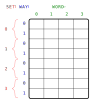
\includegraphics[width=.5\textwidth]{cache_logic_structure}
	\caption{Cache logic structure.}
	\label{fig:cache_logic_structure}
\end{figure}

Whenever a word $w$ is requested there are two possibilities:
\begin{itemize}
	\item \emph{Hit}: $w$ is present in the cache: the request can be
		immediately fulfilled.
	\item \emph{Miss}: $w$ is not present in the cache: it is necessary to
		retrieve it from lower level memory before fulfilling the
		request.
\end{itemize}
During the data retrieving a cache line is filled with a block of contiguous
words loaded from the lower level memory, trying to exploit spatial locality of
future accesses, while mapping policies and replacement policies determine which
cache line to overwrite, trying to exploit temporal locality.

If the cache memory is writable, data consistency is ensured by a consistency
policy.
\subsection{Policies}
\subsubsection{Mapping policy}
The mapping policy is in charge of statically associating a lower level memory
line to a cache set.

The \emph{set associative} policy is the most common mapping policy: given a
cache memory with $s$ sets of $w$ words, the word address (referred to the lower
level memory) bits are split into three parts (as shown in
Figure~\ref{fig:address_partitioning}):
\begin{enumerate}
	\item $\log_2(w)$: offset of the word in the line.
	\item $\log_2(s)$: set.
	\item remaining MSBs: tag identifying the specific line.
\end{enumerate}

\begin{figure}
	\centering
	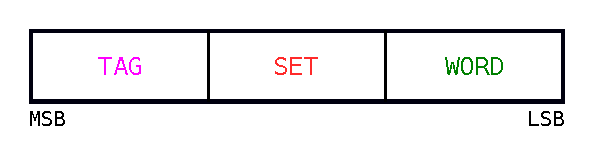
\includegraphics[width=.5\textwidth]{address_partitioning}
	\caption{Set associative policy address bits meaning.}
	\label{fig:address_partitioning}
\end{figure}

Special cases of this policy are:
\begin{itemize}
	\item \emph{Direct mapped} policy: each set is composed of a single
		line: the set bits identify a specific cache line, therefore
		there is no need for a replacement policy.
	\item \emph{Fully associative} policy: there is only a single set,
		therefore the line is fully determined by the replacement
		policy.
\end{itemize}

\subsubsection{Replacement policy}
The replacement policy is in charge of dynamically associating a lower level
memory line to a cache line of a set.

Multiple solutions of this problem have been developed, trying to maximize
the temporal locality exploitation.
Among the most commonly used solutions there are:
\begin{itemize}
	\item \emph{\acl{fifo}}: the line to be replaced is the first
		one that has been inserted to the cache.
	\item \emph{\acl{lru}}: the line to be replaced is the one
		that has least recently been accessed.
\end{itemize}

\subsubsection{Consistency policy}
The consistency policy is in charge of ensuring data consistency between
memories belonging to different hierarchy levels.

The most common solutions to this problem are:
\begin{itemize}
	\item \emph{Write-back}: write accesses are performed to the highest
		level memory and lower level memories are updated when the cache
		line is replaced only.
	\item \emph{Write-through}: each write access is propagated along the
		whole hierarchy.
\end{itemize}

\section{\acl{fpga}}
\aclp{fpga} are integrated circuits able to implement special purpose circuits
described in \ac{hdl}, thanks to their programmable logic blocks and
interconnections.
\subsection{Memory system}
An \ac{fpga} memory system is typically made up of:
\begin{itemize}
	\item registers: the fastest but most expensive memories, therefore
		they are only a few.
	\item \acp{bram}: on chip \acp{ram} accessible through simple and fast
		interface.
	\item external \acp{dram}: off chip \acp{dram} accessible through
		complex and slow interface (e.g. \acs{axi}).
\end{itemize}

\section{\acl{hls}}
\acf{hls} is an Electronic Design Automation technique aimed at translating an
algorithm description in an high-level \acl{sw} programming language (such as C
and C++) into an \ac{hdl} description.

\ac{hls} allows to design more complex systems in less time, compared to
\ac{hdl} design, moreover makes the \acl{hw} and \acl{sw} co-design much
easier, at the cost of less low-level control.


\emph{Vitis\texttrademark HLS}~\cite{vitisug} is one of the available \ac{hls}
commercial tools.

\subsection{Workflow}
The typical \ac{hls} workflow consists of:
\begin{enumerate}
	\item \emph{\ac{sw} implementation}: the top level entity is a C
		function: the function arguments are the entity ports and the
		functionality is implemented in \ac{sw}; in order to guarantee
		synthesizability some constraints should be respected (e.g.\ no
		dynamic memory allocation).
	\item \emph{\ac{sw} verification}: the testbench can be developed as a
		simple main function which calls the top level entity function,
		therefore the functionality is verified like any \ac{sw}: it is
		possible to exploit traditional tools (e.g.\ debuggers, print
		statements\ldots).
	\item \emph{\ac{hw} synthesis}: the synthesizer generates a \ac{rtl}
		description of the top level entity. It is possible to generate
		different architectures by setting up some parameters through
		dedicated directives.
	\item \emph{\ac{hw} verification}: the \ac{rtl} description is
		simulated, to make sure that \ac{sw} and \ac{hw} outputs match.
\end{enumerate}

\subsection{Optimization techniques}
Typical optimization techniques used by \ac{hls} for improving performance
include:
\begin{itemize}
	\item \textbf{Pipelining}: loops and functions logic can be pipelined
		so that successive iterations/calls can start while previous
		ones are still running. The introduced parallelism allows to
		increase the throughput at a limited additional area cost (only
		pipeline registers and a \acs{fsm} are required).
	\item \textbf{Dataflow}: different functions composing the design are
		called in a pipelined fashion (similarly to pipelining, but at
		task level, instead of instruction level).
	\item \textbf{Loop unrolling}: the loop logic is instantiated multiple
		times, to execute multiple loop iterations in parallel,
		reducing latency and improving throughput.
	\item \textbf{Memory optimizations}:
		\begin{itemize}
			\item \underline{On-chip memory:}
				\begin{itemize}
					\item \emph{Array partitioning}:
						given a factor $f$, an array is
						split into $f$ portions, each
						one mapped to a dedicated
						memory element, allowing more
						accesses to the same array at
						the same time, at the cost of
						higher memory elements usage.
						It can be block: each portion
						contains contiguous elements;
						cyclic: each portion contains
						interleaved elements.
				\end{itemize}
			\item \underline{Off-chip memory}:
				\begin{itemize}
					\item \emph{Bursting}: multiple memory
						accesses are aggregated to
						reduce overall latency and
						improving throughput.
					\item \emph{Interface widening}:
						multiple data elements are
						packed into a single bigger
						word, to perform multiple
						accesses at the same time.
				\end{itemize}
		\end{itemize}
\end{itemize}

\iffalse
\section{\texttt{C++14}}
\subsection{Templates}
\texttt{C++} templates are a special kind of classes and functions arguments
which can be of any type (even type specifiers) and are evaluated at compile
time.
This mechanism allows to write generic code: the actual values are automatically
replaced before compilation, similarly to ``\texttt{\#define}'' preprocessor
directives.

\bigskip

\subsection{Assertions}
\fi

\section{Previous work}\label{sec:liang}
Liang Ma et al.\ proposed an inlined cache implementation~\cite{liang} in the
form of \texttt{C++} classes: each of them implements an access type (read
only, write only and read write) and a mapping policy (direct mapped and set
associative).

Each cache is associated with a specific array stored to off-chip \ac{dram} and
stores its data to on-chip \acp{bram} and registers. Since the cache is
dedicated to a specific array and the accesses to a single array are usually
regular it is in general easy to tune the different parameters to get high hit
ratios.

The \texttt{operator[]} has been overloaded such that the cache can be used in
the same way of arrays, allowing to reduce the coding efforts when integrating
the cache in an existing algorithm.

During the synthesis the cache is inlined in the user algorithm: this may
clutter the logic and limit the maximum achievable performance.

\chapter{Basic architecture}
The \emph{Basic architecture} consists in a cache whose logic is separate from
application logic since it runs in a distinct process
(Figure~\ref{fig:single_proc_basic_arch}).
It starts from same assumptions of Ma's architecture (introduced in
Section~\ref{sec:liang}): accelerate accesses to off-chip \ac{dram} arrays
associating them with dedicated caches which store their data to on-chip
\ac{bram} and registers.

The acceleration is achieved by:
\begin{itemize}
	\item \underline{optimizing \ac{axi} accesses:} the cache aggregates
		\ac{dram} accesses in lines, allowing to exploit automatic port
		widening and burst accesses.
	\item \underline{reducing \ac{axi} accesses:} the \ac{axi} interface is
		accessed in case of cache miss only.
\end{itemize}

The \emph{Basic architecture} is aimed at solving the main limitation of Ma's
one: inlining the cache into application makes the logic more complex and the
synthesis may not be able to generate a circuit with optimal performance.

Since the cache process is isolated from the application logic, it should
always perform in the same manner, independently from the algorithm in which it
is used, while the algorithm may get better performance, since it would only
contain \ac{fifo} accesses instead of the whole cache logic.

\begin{figure}
	\centering
	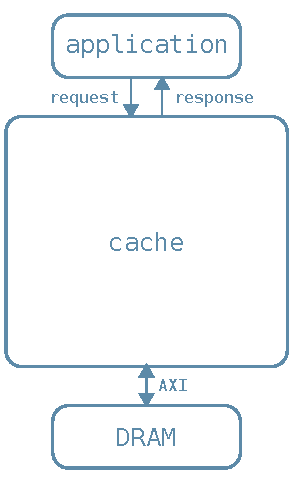
\includegraphics[width=.3\textwidth]{single_proc_basic_arch}
	\caption{\emph{Single-process Basic architecture} overview.}
	\label{fig:single_proc_basic_arch}
\end{figure}

\paragraph{Functionality}
If application $A$ needs to access the array associated with the cache $C$:
\begin{enumerate}
	\item $A$ writes the request to the request \ac{fifo}.
	\item $C$ reads the request \ac{fifo} and checks if the requested
		address causes a miss.
	\item (in case of miss) $C$ issues a request to the \ac{axi} interface
		to prepare its own memory (mapped to \ac{bram}) for fulfilling
		the requested access.
	\item $C$ performs the access to \ac{bram} and (in case of read
		request) writes requested data to the response \ac{fifo}.
	\item (in case of read request) $A$ reads requested data from the
		response \ac{fifo}.
\end{enumerate}

\paragraph{Characteristics}
The \emph{Basic architecture} is compliant with the set associative mapping
policy and the write-back consistency policy.
It is configurable in terms of:
\begin{itemize}
	\item Word type and number of words per line.
	\item Number of sets and ways (therefore it is possible to obtain a
		fully associative policy by setting the number of sets to 1 or
		a direct mapped policy by setting the number of ways to 1).
	\item Replacement policy (\acl{lru} or \acl{fifo}).
\end{itemize}

\paragraph{Single-process and Multi-processes Basic architectures}
The \emph{Single-process Basic architecture} is composed of a single pipelined
process which performs all the cache functionalities.

This process can be pipelined with an \ac{ii} of 1 when memory accesses are
Read-Only and a cache line is not bigger than the maximum \ac{axi} interface
width (512 or 1024 bits typically, depending on the specific device).

Write accesses generate some dependencies on the \ac{axi} interface, while large
cache lines require multiple \ac{axi} transactions since they do not fit a
single one: both of these increase the process \ac{ii}, worsening cache
performance.

\bigskip
The \emph{Multi-processes Basic architecture} splits cache into two processes
(Figure~\ref{fig:multi_proc_basic_arch}):
\begin{itemize}
	\item \emph{core} process: manages communication with application and
		keeps cache data structures up to date.
	\item \emph{memory interface} process: deals with the \ac{axi}
		interface.
\end{itemize}

This architecture is aimed at solving the performance limitations of the
\emph{Single-process Basic architecture} in case of writable caches: it manages
to pipeline the \emph{core} process with an \ac{ii} of 1, even in case of write
accesses or long lines, since the \ac{axi} interfacing resides in the separate
\emph{memory interface} process.

The latency of the response to an hitting request depends on the \emph{core}
process only, therefore with this solution best performance is achieved in case
of writable caches too.

\begin{figure}
	\centering
	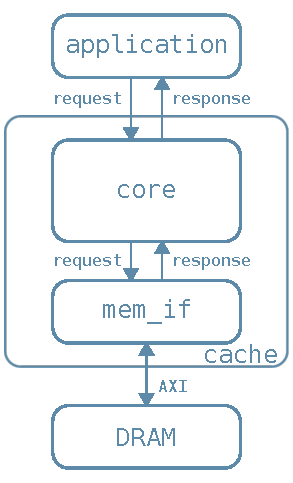
\includegraphics[width=.3\textwidth]{multi_proc_basic_arch}
	\caption{\emph{Multi-processes Basic architecture} overview.}
	\label{fig:multi_proc_basic_arch}
\end{figure}

\section{Implementation}
The \emph{Basic architecture} is implemented in the form of a
\texttt{C++14}~\cite{cpp14} class, compatible with
\emph{Vitis\texttrademark~HLS~2021.1}.
All the configurable parameters are set through class template arguments.

The cache class is logically split into two parts:
\begin{itemize}
	\item \emph{Internals}: cache functionalities.
	\item \emph{Interface}: \acsp{api} for managing requests and responses
		from application side.
\end{itemize}

\subsection{Internals}
The \emph{Internals} implementation differs between the \emph{Single-process}
and the \emph{Multi-processes} implementations:
\begin{itemize}
	\item \emph{Single-process Basic architecture}: single process which
		implements all the cache functionalities.
	\item \emph{Multi-processes Basic architecture}:
		\begin{itemize}
			\item \emph{core} process: same as \emph{Single-process
				Basic architecture} process, but it does not
				directly accesses the \ac{axi} bus: it issues
				requests to the \emph{memory interface} process
				through \acp{fifo}.
			\item \emph{memory interface} process: it accesses the
				\ac{axi} bus as requested by the \emph{core}
				process.
		\end{itemize}
\end{itemize}

\subsubsection{Array partitioning}
Cache memory (which stores the actual data) must be accessed one line per clock
cycle: it is mapped to a \ac{bram} array cyclically partitioned with a factor
equal to the number of lines.

Helper data (e.g. \texttt{tag}, \texttt{valid}, \texttt{dirty}\ldots) is stored
to completely partitioned arrays, mapped to registers, in order to avoid
dependencies as much as possible and get best performance.

\subsubsection{Process modeling}
\ac{hls} is intended for synthesizing sequential \acl{sw} code, therefore it has
been necessary to develop a novel technique for modeling multi-process designs.

A process is modeled as an infinite loop and their parallelism is modeled
differently depending on the compilation target:
\begin{itemize}
	\item \emph{\ac{sw} simulation}: each process is mapped to an
		\texttt{std::thread}.
	\item \emph{\ac{hw} synthesis}: each process is a dataflow function, in
		a dataflow region with the \texttt{disable\_start\_propagation}
		option disabled (which allow each function to run in parallel,
		without waiting for the completion of previous ones).
\end{itemize}
The distinction between simulation and synthesis code can be performed through
the ``\texttt{\#ifdef \_\_SYNTHESIS\_\_}'' preprocessor directive.

Different processes can communicate by means of \acp{fifo} (\texttt{hls::stream}
provided by Vitis\texttrademark HLS), which allow unidirectional point-to-point
communication between two processes. It is possible to insert multiple
\acp{fifo} between each process, in both directions, therefore allowing to
setup duplex communication.

Since \texttt{hls::stream} provides blocking operations, these \acp{fifo} can
be also used for synchronization purposes.

\subsubsection{\acl{raw} dependencies}
The cache process \ac{ii} is limited by the \ac{raw} dependencies on the cache
lines, therefore the \emph{\ac{raw} cache} has been developed: it is a
single-line cache which provides the functions:
\begin{itemize}
	\item \texttt{get\_line}: in case of hit, read the \emph{\ac{raw}
		cache} line; in case of miss, read the cache line.
	\item \texttt{set\_line}: write both the \emph{\ac{raw} cache} line and
		the cache line.
\end{itemize}

Cache memory is always accessed through the \emph{\ac{raw} cache} and the
\texttt{set\_line} function is called once per iteration at most: if a cache
line has been written it is impossible that it is read in the next iteration,
since the \ac{raw} cache would hit and return its line. This allows to falsify
the \ac{raw} dependency of distance of 1 on the cache memory, making it
possible to schedule the cache process with an \ac{ii} of 1.

\subsubsection{Conditional code compilation}
\emph{Single-process Basic architecture} provides better performance and lower
resource usage (with respect to the \emph{Multi-processes} one) when it is
possible to schedule its process with an \ac{ii} of 1 (read-only accesses with
line not larger than the maximum \ac{axi} interface bitwidth): therefore it is
automatically instantiated whenever it is convenient.

Alternatively executing the \emph{Multi-processes} or the \emph{Single-process}
code with traditional \texttt{if} statements would generate errors during the
synthesis, particularly in the \emph{Dataflow check} step (which checks that
each \texttt{hls::stream} has a single reader and a single writer): the
compiler builds both branches of the \texttt{if} statements, independently from
the fact that one of them is never executed.

The problem can be solved through the \ac{sfinae} pattern, which allows to make
the compiler ignore parts of code when the template substitution is invalid,
instead of throwing an error.
This technique can be easily implemented by using the \texttt{std::enable\_if}
structure which conditionally returns an invalid type, triggering the
\ac{sfinae} pattern.

\subsection{Interface}
Provide \acsp{api} for managing requests and responses from application to
cache:
\begin{itemize}
	\item \texttt{get}: send a read request and read the response.
	\item \texttt{set}: send a write request.
\end{itemize}
To improve user friendliness, similarly to Ma's implementation, the
\texttt{operator[]} has been overloaded so that a cache object can be used as a
traditional array (e.g. \texttt{val~=~cache[i]} calls
\texttt{val~=~cache.get(i)} and \texttt{cache[i]~=~val} calls
\texttt{cache.set(i,~val)}).

\iffalse
\begin{table}
	\begin{center}
		\begin{tabularx}{\textwidth}{LCC}
			\hline
			\rowcolor{gray!50}
			& \textbf{Single-process basic implementation} &
			\textbf{Ma's implementation} \\
			\hline
			\textbf{Integration with algorithm} & Separate process &
			Inlined \\
			\rowcolor{gray!25}
			\textbf{Underlying memory} & Single \ac{dram} array &
			Single \ac{dram} array \\
			\textbf{Configurability} & Template arguments &
			Template arguments and dedicated classes \\
			\rowcolor{gray!25}
			\textbf{\texttt{operator[]} overload} & Array-like &
			Array-like \\
			\hline
		\end{tabularx}
	\end{center}
	\caption{Comparison between basic single-process and Ma's
	implementations.}
	\label{tab:basic_vs_liang}
\end{table}
\fi

\chapter{Optimized architectures}
\section{\ac{l1} cache}
Each \ac{fifo} access costs one clock cycle, which has to be paid for each
memory access.
To improve performance each read request to the cache does not return a single
data element, but a whole cache line. This allows to insert a \ac{l1} cache
above the underlying cache, directly inlined in the user logic
(Figure~\ref{fig:l1_arch}), similarly to Ma's architecture.

An equivalent approach could have been applied to write requests, but given that
read accesses are usually more frequent than write accesses, therefore more
sensitive to optimizations and that it is crucial not to clutter the user
logic, the \ac{l1} cache is kept as simple as possible: it complies with the
write-through consistency policy, which is simpler but does not provide any
advantage to write accesses.

To keep up with simplicity the \ac{l1} cache is direct-mapped.

\begin{figure}
	\centering
	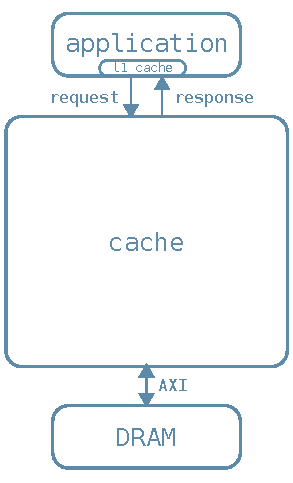
\includegraphics[width=.3\textwidth]{l1_arch}
	\caption{Cache architecture optimized with the insertion of a \ac{l1}
	cache.}
	\label{fig:l1_arch}
\end{figure}

\subsection{Implementation}
The \ac{l1} cache has been added to the \emph{Basic architecture} through a few
modifications:
\begin{itemize}
	\item the template argument determining the number of \ac{l1} cache
		lines has been added.
	\item the data \ac{fifo} from cache to algorithm has been extended to
		fit a whole cache line.
	\item the \texttt{get} function, instead of directly issuing the read
		request to the \ac{l2} cache, it checks if the \ac{l1} cache
		hits: if so it reads the data from the \ac{l1} cache, otherwise
		it issues the request to the \ac{l2} cache.
	\item the \texttt{set} function sets the \ac{l1} cache line to dirty.
\end{itemize}

\section{Multiple ports}
The vast majority of algorithms accesses memory inside loops, which in \ac{hls}
can be optimized in two main ways: pipelining, which perfectly fits the
single-port cache architecture, and unrolling, with which the \ac{ii} would
increase, since each unrolled iteration should access the same \ac{fifo} at the
same time.

To solve this problem a multi-port architecture is proposed: each port has
dedicated \acp{fifo} and the cache process serves each request in order.
Each port has also a dedicated \ac{l1} cache, which can be used without any
coherency problem, since they follow the write-through consistency policy.

\subsection{Implementation}
\subsubsection{Port binding}


\chapter{Results}
\section{Matrix multiplication}
\section{Bitonic sorting}
\section{Lucas-Kanade}

\chapter{Conclusion}

\backmatter

\printbibliography

\end{document}

